%%%% SEITENRAENDER, SCHRIFTGROESSE UND ZEILENABSTAND NICHT ABAENDERN => SONST GIBT ES PUNKTEABZUG
\documentclass[a4paper,11pt,singlespacing]{article}
% \usepackage[left=2.5cm,right=2.5cm,top=2.5cm]{geometry}
\usepackage{setspace}
\usepackage[utf8]{inputenc}
\usepackage{graphicx}
\usepackage{color}
\usepackage{hyperref}
\usepackage{biblatex}
\usepackage{listings}
\usepackage{xcolor}
\usepackage{float}

\definecolor{codegreen}{rgb}{0,0.6,0}
\definecolor{codegray}{rgb}{0.5,0.5,0.5}
\definecolor{codepurple}{rgb}{0.58,0,0.82}
\definecolor{backcolour}{rgb}{0.95,0.95,0.92}

\lstdefinestyle{mystyle}{
    backgroundcolor=\color{backcolour},   
    commentstyle=\color{codegreen},
    keywordstyle=\color{magenta},
    numberstyle=\tiny\color{codegray},
    stringstyle=\color{codepurple},
    basicstyle=\ttfamily\footnotesize,
    breakatwhitespace=false,         
    breaklines=true,                 
    captionpos=b,                    
    keepspaces=true,                 
    numbers=left,                    
    numbersep=5pt,                  
    showspaces=false,                
    showstringspaces=false,
    showtabs=false,                  
    tabsize=2
}

\lstset{style=mystyle}

\addbibresource{sample.bib}


\usepackage{listings,xcolor}
%opening
\title{Project title}
\author{
	Name Mat.No.
	}


\begin{document}
% Absatzeinrückung verhindern
\setlength{\parindent}{0ex}


\begin{titlepage}
	
	\newcommand{\HRule}{\rule{\linewidth}{0.5mm}} % Defines a new command for the horizontal lines, change thickness here
	
	\center % Center everything on the page
	
	%----------------------------------------------------------------------------------------
	%	HEADING SECTIONS
	%----------------------------------------------------------------------------------------
	
	\textsc{\LARGE University of Applied Sciences Ravensburg Weingarten}\\[1.5cm] % Name of your university/college
	\textsc{\Large Department of
		Electrical Engineering
		and Computer Science}\\[0.5cm] % Major heading such as course name
	\textsc{\large Computer Science Project}\\[0.5cm] % Minor heading such as course title
	
	%----------------------------------------------------------------------------------------
	%	TITLE SECTION
	%----------------------------------------------------------------------------------------
	
	\HRule \\[0.4cm]
	{ \huge \bfseries Prototype of a autonomous selfi drone utilizing pose estimation}\\[0.4cm] % Title of your document
	\HRule \\[1.5cm]
	
	%----------------------------------------------------------------------------------------
	%	AUTHOR SECTION
	%----------------------------------------------------------------------------------------
	
	\begin{minipage}{0.4\textwidth}
		\begin{flushleft} \large
			\emph{Author:}\\
			Felix \textsc{Hamburger}\\ % Your name
			28403
		\end{flushleft}
	\end{minipage}
	~
	\begin{minipage}{0.4\textwidth}
		\begin{flushright} \large
			\emph{Supervisor:} \\
			Prof. Dr. Markus \textsc{Schneider} % Supervisor's Name
		\end{flushright}
	\end{minipage}\\[2cm]

	% If you don't want a supervisor, uncomment the two lines below and remove the section above
	%\Large \emph{Author:}\\
	%John \textsc{Smith}\\[3cm] % Your name
	
	%----------------------------------------------------------------------------------------
	%	DATE SECTION
	%----------------------------------------------------------------------------------------
	
	{\large \today}\\[5cm] % Date, change the \today to a set date if you want to be precise
	
	%----------------------------------------------------------------------------------------
	%	LOGO SECTION
	%----------------------------------------------------------------------------------------
	
	
	
\includegraphics[width=7cm]{images/logo.png} % Include a department/university logo - this will require the graphicx package
	
	%----------------------------------------------------------------------------------------
	
	\vfill % Fill the rest of the page with whitespace
	
\end{titlepage}


\tableofcontents
\pagebreak


%%%%%%%%%%%%%%%%%%%%%%%%%%%%%%% Introduction
\section{Introduction}
Drones have long since arrived in the living rooms of ordinary households. They are no longer just dreams of the future that only rich tech nerds could afford.
\\\\
They are available on the market in numerous variations.
From the small indoor drone, which can fly only a few meters high, to the long-range drone that can be remotely controlled over several kilometers.
\\\\
They vary from manually controlled drones to completely autonomous systems that only need to be turned on to do their job.
\\\\
In this project I would like to develop an autonomous prototype and gain first experiences in the field of autonomous UAVs.
The aim is to apply ready-made solutions which act together and control a drone which is autonomous and is controlled via gesture control.

\subsection{Objective}
At the beginning I would like to define some core features which have to be 
implemented in the course of the project.
\begin{itemize}
	\item The drone must be able to move autonomously and follow the oerpator.
	\item The drone must be able to be controlled by gestures.
	\item The drone must be able to take a photo of the operator.
\end{itemize}





\pagebreak
%%%%%%%%%%%%%%%%%%%%%%%%%%%%%% Requirements
\section{Requirements}
This section lists the three most important parts for this project:
\begin{itemize}
	\item \textbf{Drone:} The Tello drone used in this project.
	\item \textbf{DJITelloPy:} The library used to control the drone.
	\item \textbf{Mediapipe (BlazePose):} The Framework (CNN) used in this project.
	
\end{itemize}
\subsection{Drone}
The Tello drone from Ryze Tech is best suited for this project. Since this project is mainly 
about the combination of different ready-made solutions, the time needed to build a drone yourself would be too great.
\\\\
Ryze Tech offers with its Tello drone a complete solution under 100€ which is additionally equipped with a software development kit. 
The drone itself is small and suitable for indoor use.
\\\\
\begin{figure}[H]
	\centering
	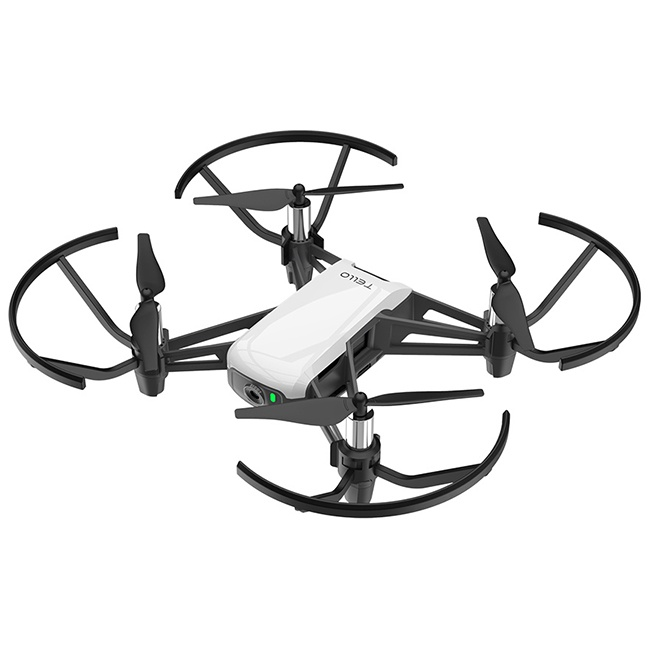
\includegraphics[scale=0.4]{images/tello_front.jpeg}
	\caption{Tello Drone}
	\label{tello_drone}
\end{figure}

The following table provides a clear overview of the technical details:

\begin{center}
	\begin{tabular}{ l  l} 
	\hline
	 \textbf{Aircraft:} & Weight: 80g\\
	 & Dimensions: 98×92.5×41 mm  \\
	 & Propeller: 7,62cm\\
	 & Built-in Functions: Range Finder,\\
	 & Barometer, LED, Vision System,\\
	 & 2.4 GHz 802.11n Wi-Fi, 720p Live View\\
	 & Port: Micro USB Charging Port\\\\
	 \hline
	\\
	 \textbf{Flight Performance:} & Max Flight Distance: 100m\\
	 & Max Speed: 8m/s\\
	 & Max Flight Time: 13min\\
	 & Max Flight Height: 30m\\\\
	 \hline
	 \\
	 \textbf{Battery:} & Detachable Battery: 1.1Ah/3.8V\\\\
	 \hline
	 \\
	 \textbf{Camera:} & Photo: 5MP (2592x1936)\\
	 & FOV: 82.6° \\
	 & Video: HD720P30\\
	 & Format: JPG(Photo); MP4(Video)\\
	 & Electric Image Stabilization: Yes\\
	 \hline
	\end{tabular}
\end{center}



\subsection{Tello SDK}

The Tello SDK\cite{TelloSDK} is the official software development kit for the Tello drone. 
The SDK connects the drone via Wifi to a UDP port and lets the user control it via
text commands.
\\
During startup of the drone, it opens up a Wi-Fi channel, where the drone can be 
reached under the IP address IP 192.168.10.1.\\

The drone communicates and receives messages over three different ports:\\
\begin{itemize}
	\item \textbf{UDP PORT:8889}: The drone will receive commands over this port.
	\item \textbf{UDP PORT:8890}: The drone will send its state to this port.
	\item \textbf{PORT:11111}: The drone will send the video stream to this port.
\end{itemize}

The SDK includes three basic command types:\\\\
\textbf{Control Commands:} Command to send a movement text command to the drone. It will return \textit{ok} if the command was succesfully executed 
and \textit{error} if the command is unsuccesful.\\\\
\textbf{Read Commamnds:} Command to request parameters like batterylevel. It will return the parameters of the requested parameters.\\\\
\textbf{Set Commands:} Command to set parameters like the drones speed. It will return \textit{ok} if the command was succesfully executed 
and \textit{error} if the command is unsuccesful.

\begin{center}
	\begin{tabular}{c | c | c} 
	\hline
	 Command & Description & Possible response\\
	 \hline
	 takeoff & Tello auto takeoff & ok, error \\
	 streamon & Set video stream on & ok,error\\
	 right & fly right x centimeters & ok,error\\
	 battery? & get current battery level in percent & 0-100\\
	\end{tabular}
\end{center}

The Tello SDK itself offers a variety of different commands which would be 
sufficient for operating the drone both autonomously and via poses.

\subsubsection{DJITelloPy}

DJITelloPy\cite{DJITelloPy} utilizes the Tello SDK and provides similar commands which ulimately
build on the commands of the Tello SDK.
\\\\
But concerning the video streaming, the Tello SDK canbe quite tricky because 
someone has to parse the udp stream itself to receive the neccesary video data.
\\
DJITelloPy offers an easy solution for video streaming with return values 
which can be directly used with OpenCV.

\subsection{Mediapipe}
Mediapipe\cite{Mediapipe} is an open source framework from Gogle which offers a 
variety of machine learning solutions.

One of its solutions is its pose estimation which is a high-fidelity body pose tracking capable of tracking 33 3D Landmarks.+
Mediapipe Pose utiliuzes the BlazePose\cite{BlazePosePaper} Convolutional Neural Network which will be described in the following section.

\subsubsection{Pose}

The Pose Solution from Mediapipe operates in two steps.
First the person including two additional keypoints are detected that allow to describe the 
describe the human body center, rotation and scale as a circle.
Then the BlazePose model predicts the location of 33 3D Landmarks as seen in the following image.

\begin{figure}[H]
	\centering
	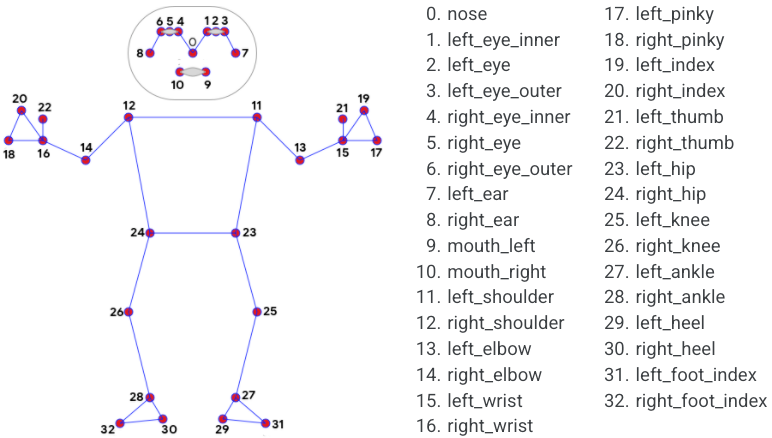
\includegraphics[width=\textwidth]{images/mediapipe_landmarks.png}
	\caption{BlazePose Landmarks}
	\label{mediapipe_landmarks}
\end{figure}

The modle outouts a list of pose landmarks which consist of:
\begin{itemize}
	\item X Coordinate of the landmark normalized from 0.0 to 1.0.
	\item Y Coordinate of the landmark normalized from 0.0 to 1.0.
	\item Z, which represents the depth of the landmark with the depth at the midpoint of hips being the origin.
	\item Visibility of the landmark with a probability from 0.0 to 1.0.
\end{itemize}

\pagebreak
%%%%%%%%%%%%%% IMplementation
\section{Implementation}
This chapter explains how the algorithm for controlling the drone works. This chapter is divided into three parts.
The first part explains how the state machine works.
The second part which explains how the drone reacts to poses.
and the third part is explaining how the drone flies autonomously.

\subsection{Algorithm}
The algorithm itself works as a state machine where each frame is evaluated 
individually based on the applied pose estimation. 

At the beginning of the loop, the frame is read and Pose Estimation is applied to the frame.
If one of the three implemented poses is detected the following steps will be initiated:
\begin{itemize}
	\item \textbf{Arms crossed:} The drone takes a picture.
	\item \textbf{Right arm up:} The drone hovers to the left (right from drone view)
	\item \textbf{Left arm iup:} The drone hovers to the right (left from drone view)
\end{itemize}

If no pose is detected in a frame, the drone hovers autonomously following the operator.

\begin{figure}[H]
	\centering
	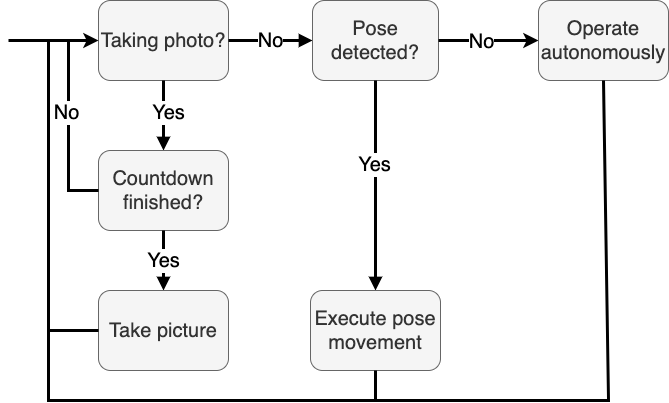
\includegraphics[width=\textwidth]{images/flow_chart_code.png}
	\caption{Flowchart of the states the drone can enter}
	\label{flowchart_code}
\end{figure}

In order to be able to follow the following explanations, it is important to mention that the recorded frames have their 
zero point in the upper left edge of the image.\\
This is shown here:

\begin{figure}[H]
	\centering
	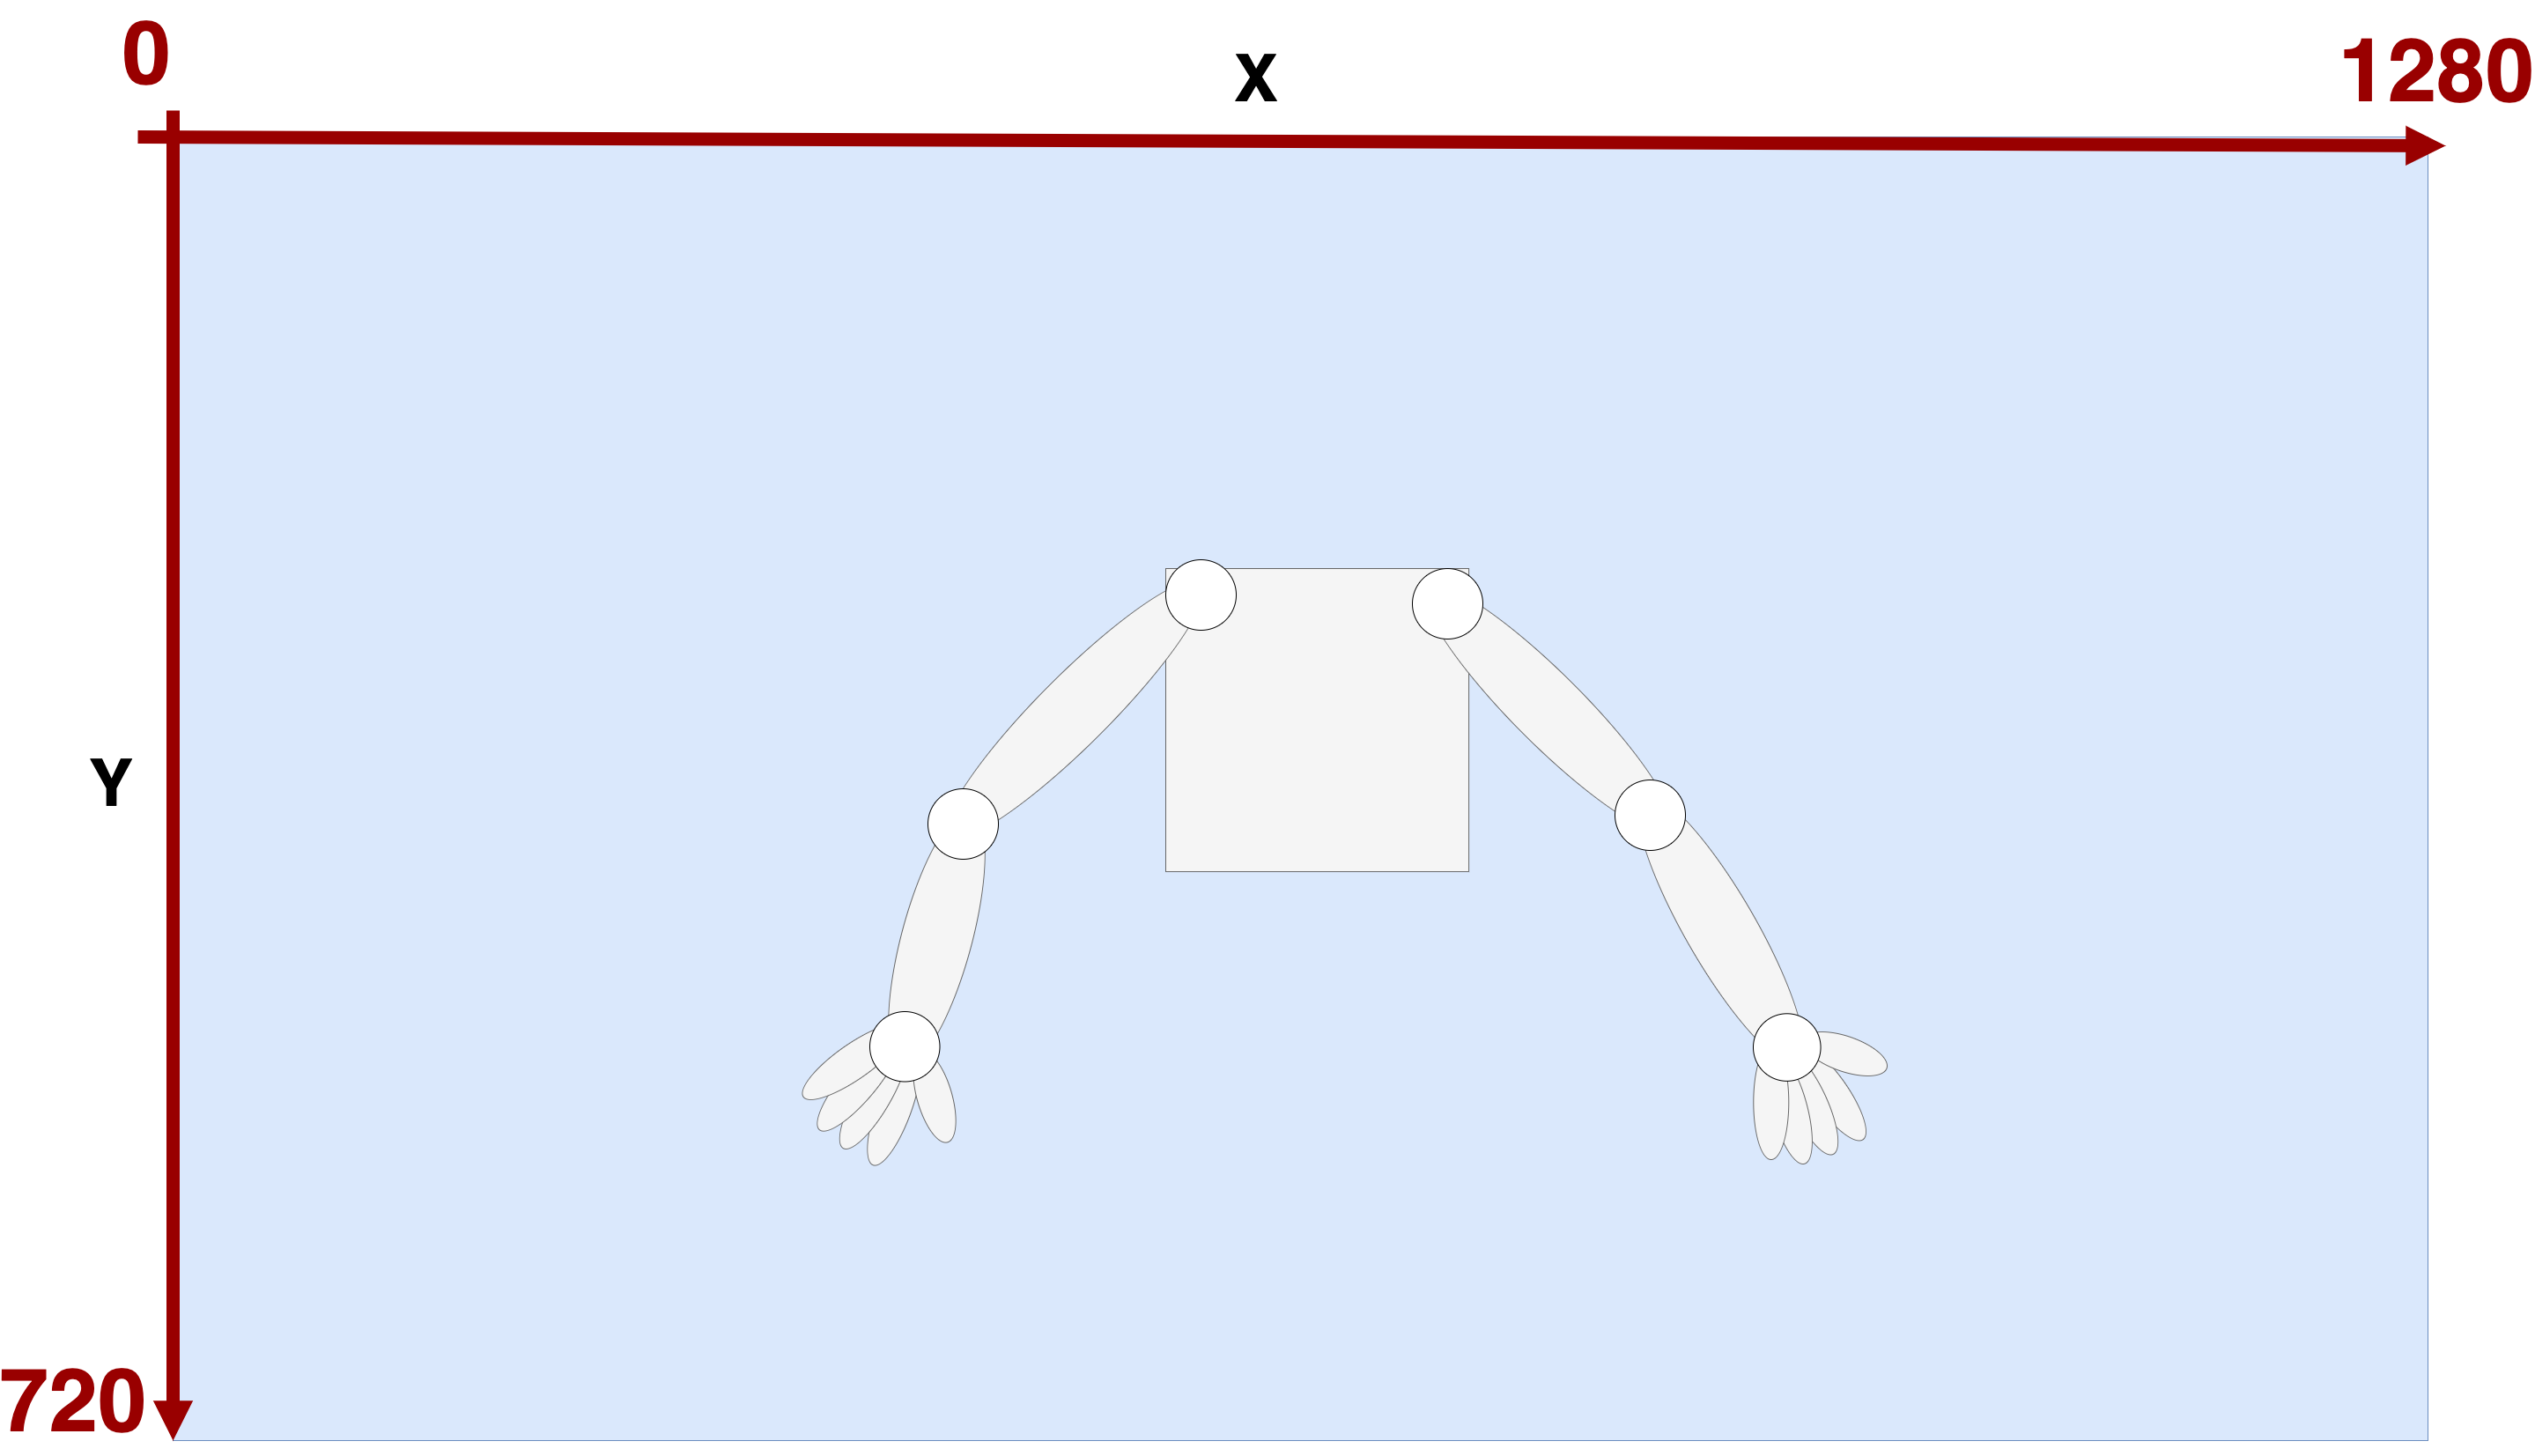
\includegraphics[width=\textwidth]{images/video_frame.png}
	\caption{Illustration of the video frame}
	\label{video_frame}
\end{figure}

It must be noted, that everything the camera captures is mirrored, thus the left arm 
in this picture correlates to the right arm in real live.
This will become more obvious when we dive into the poses in detail.
\subsection{Poses}

This chapter explains how the three poses are recognized by the drone.\\\\

To recognize the first pose four Landmakrs are needed.
\begin{itemize}
	\item Right Wrist
	\item Left Wrist
	\item Right shoulder
	\item Left Shoulder
\end{itemize}

In a normal body posture, it is assumed that the left arm or wrist is below the left shoulder landmark.
If the right wrist is now lifted above the right shoulder landmark, the drone recognizes that the right arm has been lifted.\\\\
Here it is important to note that the returned x and y components behave inversely 
since we have the zero point in the upper left edge of the screen.\\\\
This means that an arm is considered lifted if its y values are lower than the y values of the shoulder landmark.\\\\
If this pose is detected, the drone controller will give the command to fly the drone from its direction to the left.
\begin{figure}[H]
	\centering
	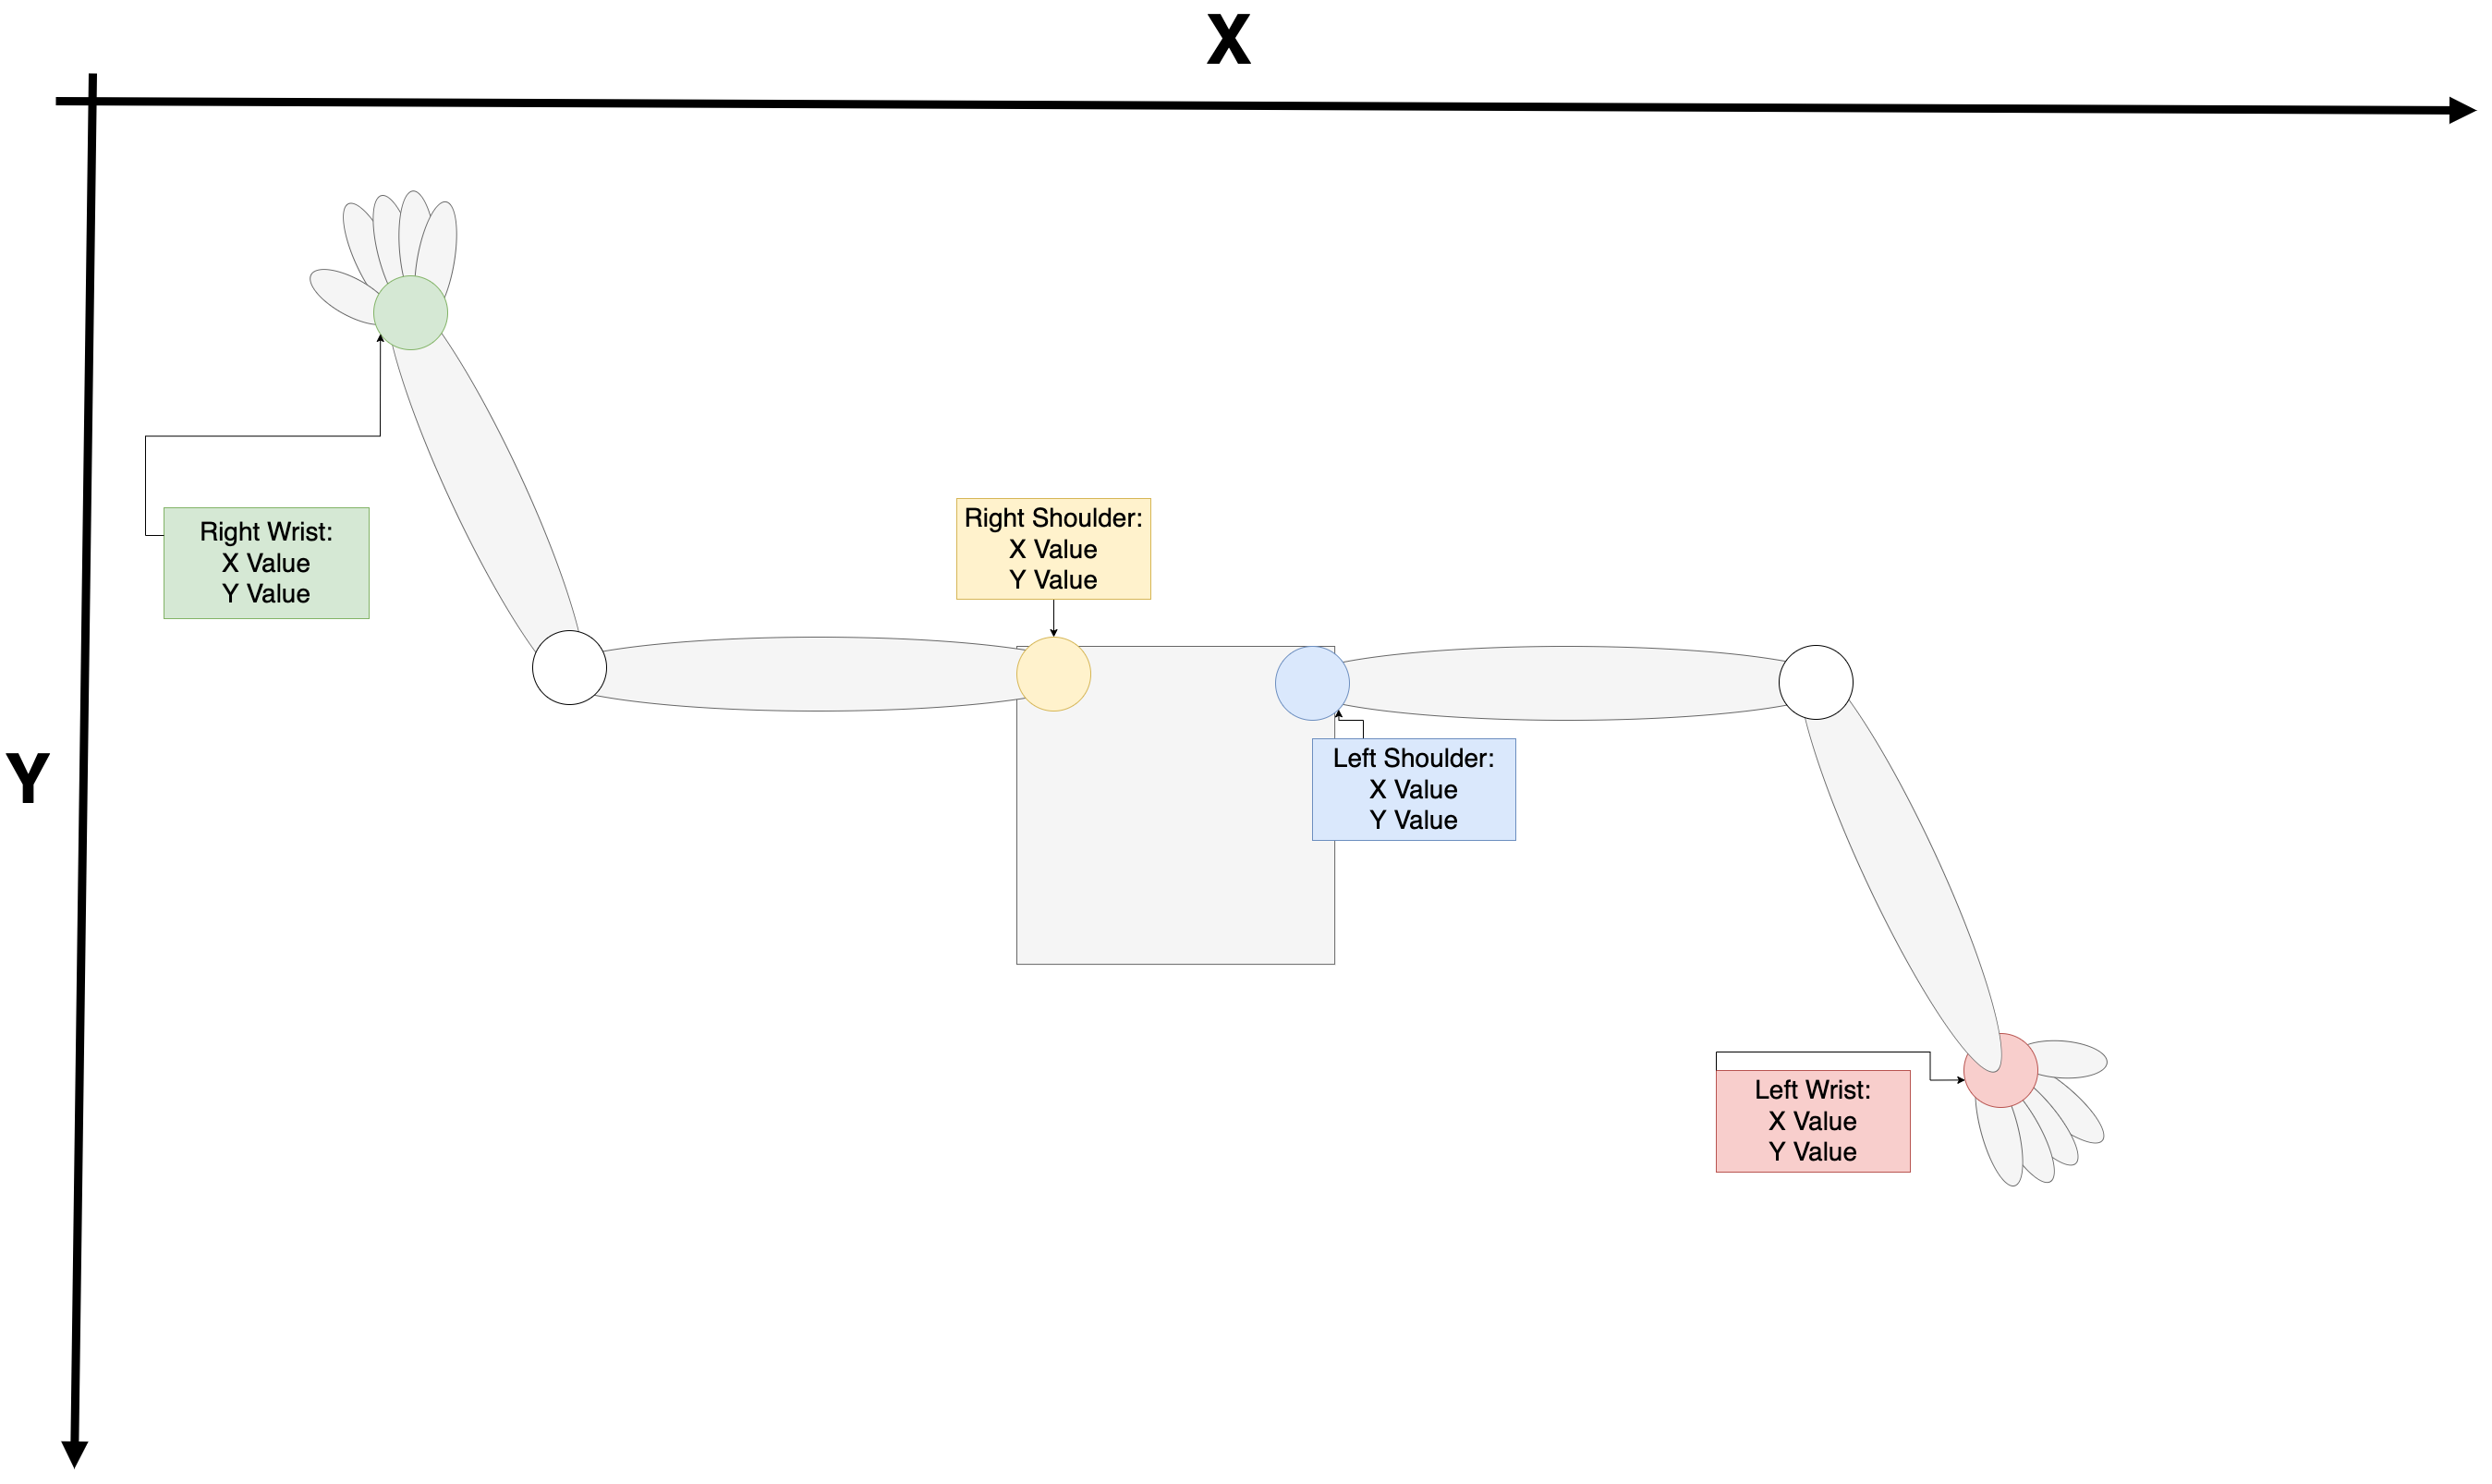
\includegraphics[width=\textwidth]{images/right_arm_up.png}
	\caption{Pictogram of the pose "right arm up"}
	\label{right_arm_up}
\end{figure}
We have a similar case when detecting the lift of the left arm. 
Here, the larger/smaller comparisons must be reversed.\\\\
If this pose is detected, the drone controller will give the command to fly the drone to the right.

\begin{figure}[H]
	\centering
	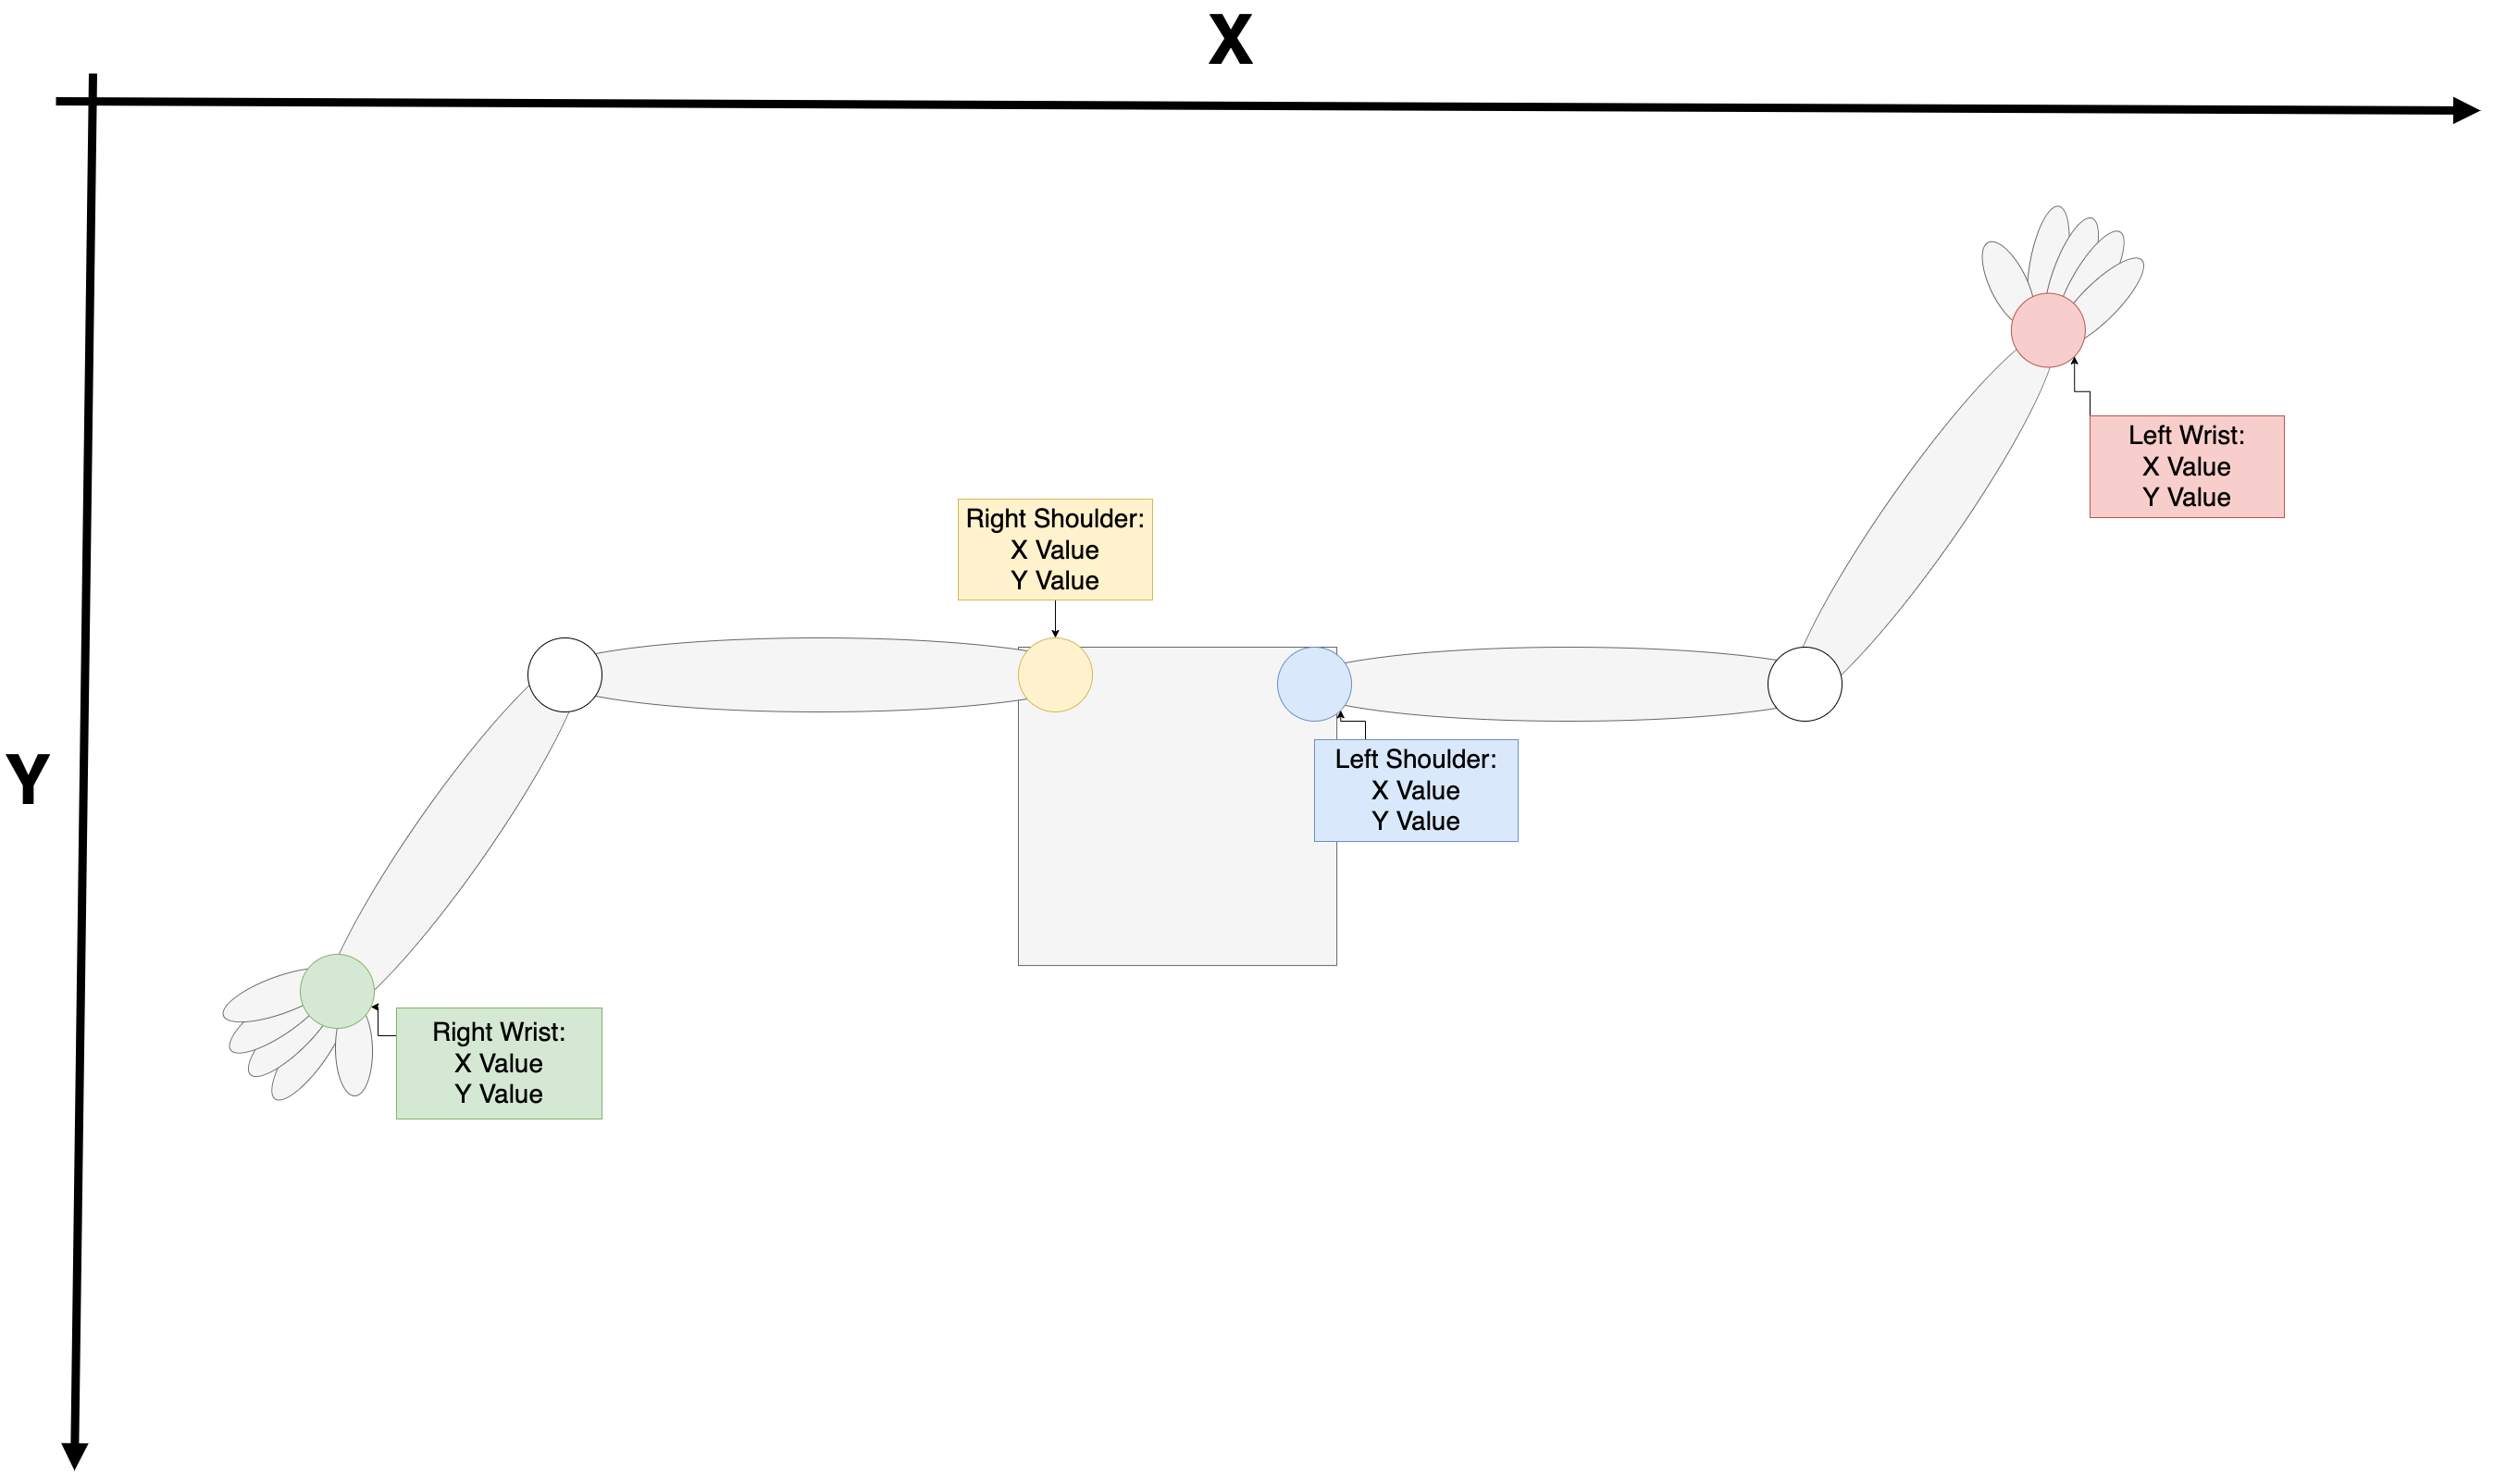
\includegraphics[width=\textwidth]{images/left_arm_up.png}
	\caption{Pictogram of the pose "left arm up"}
	\label{left_arm_up}
\end{figure}

In the third pose, the drone should detect if the arms are crossed in front of the body.

\begin{figure}[H]
	\centering
	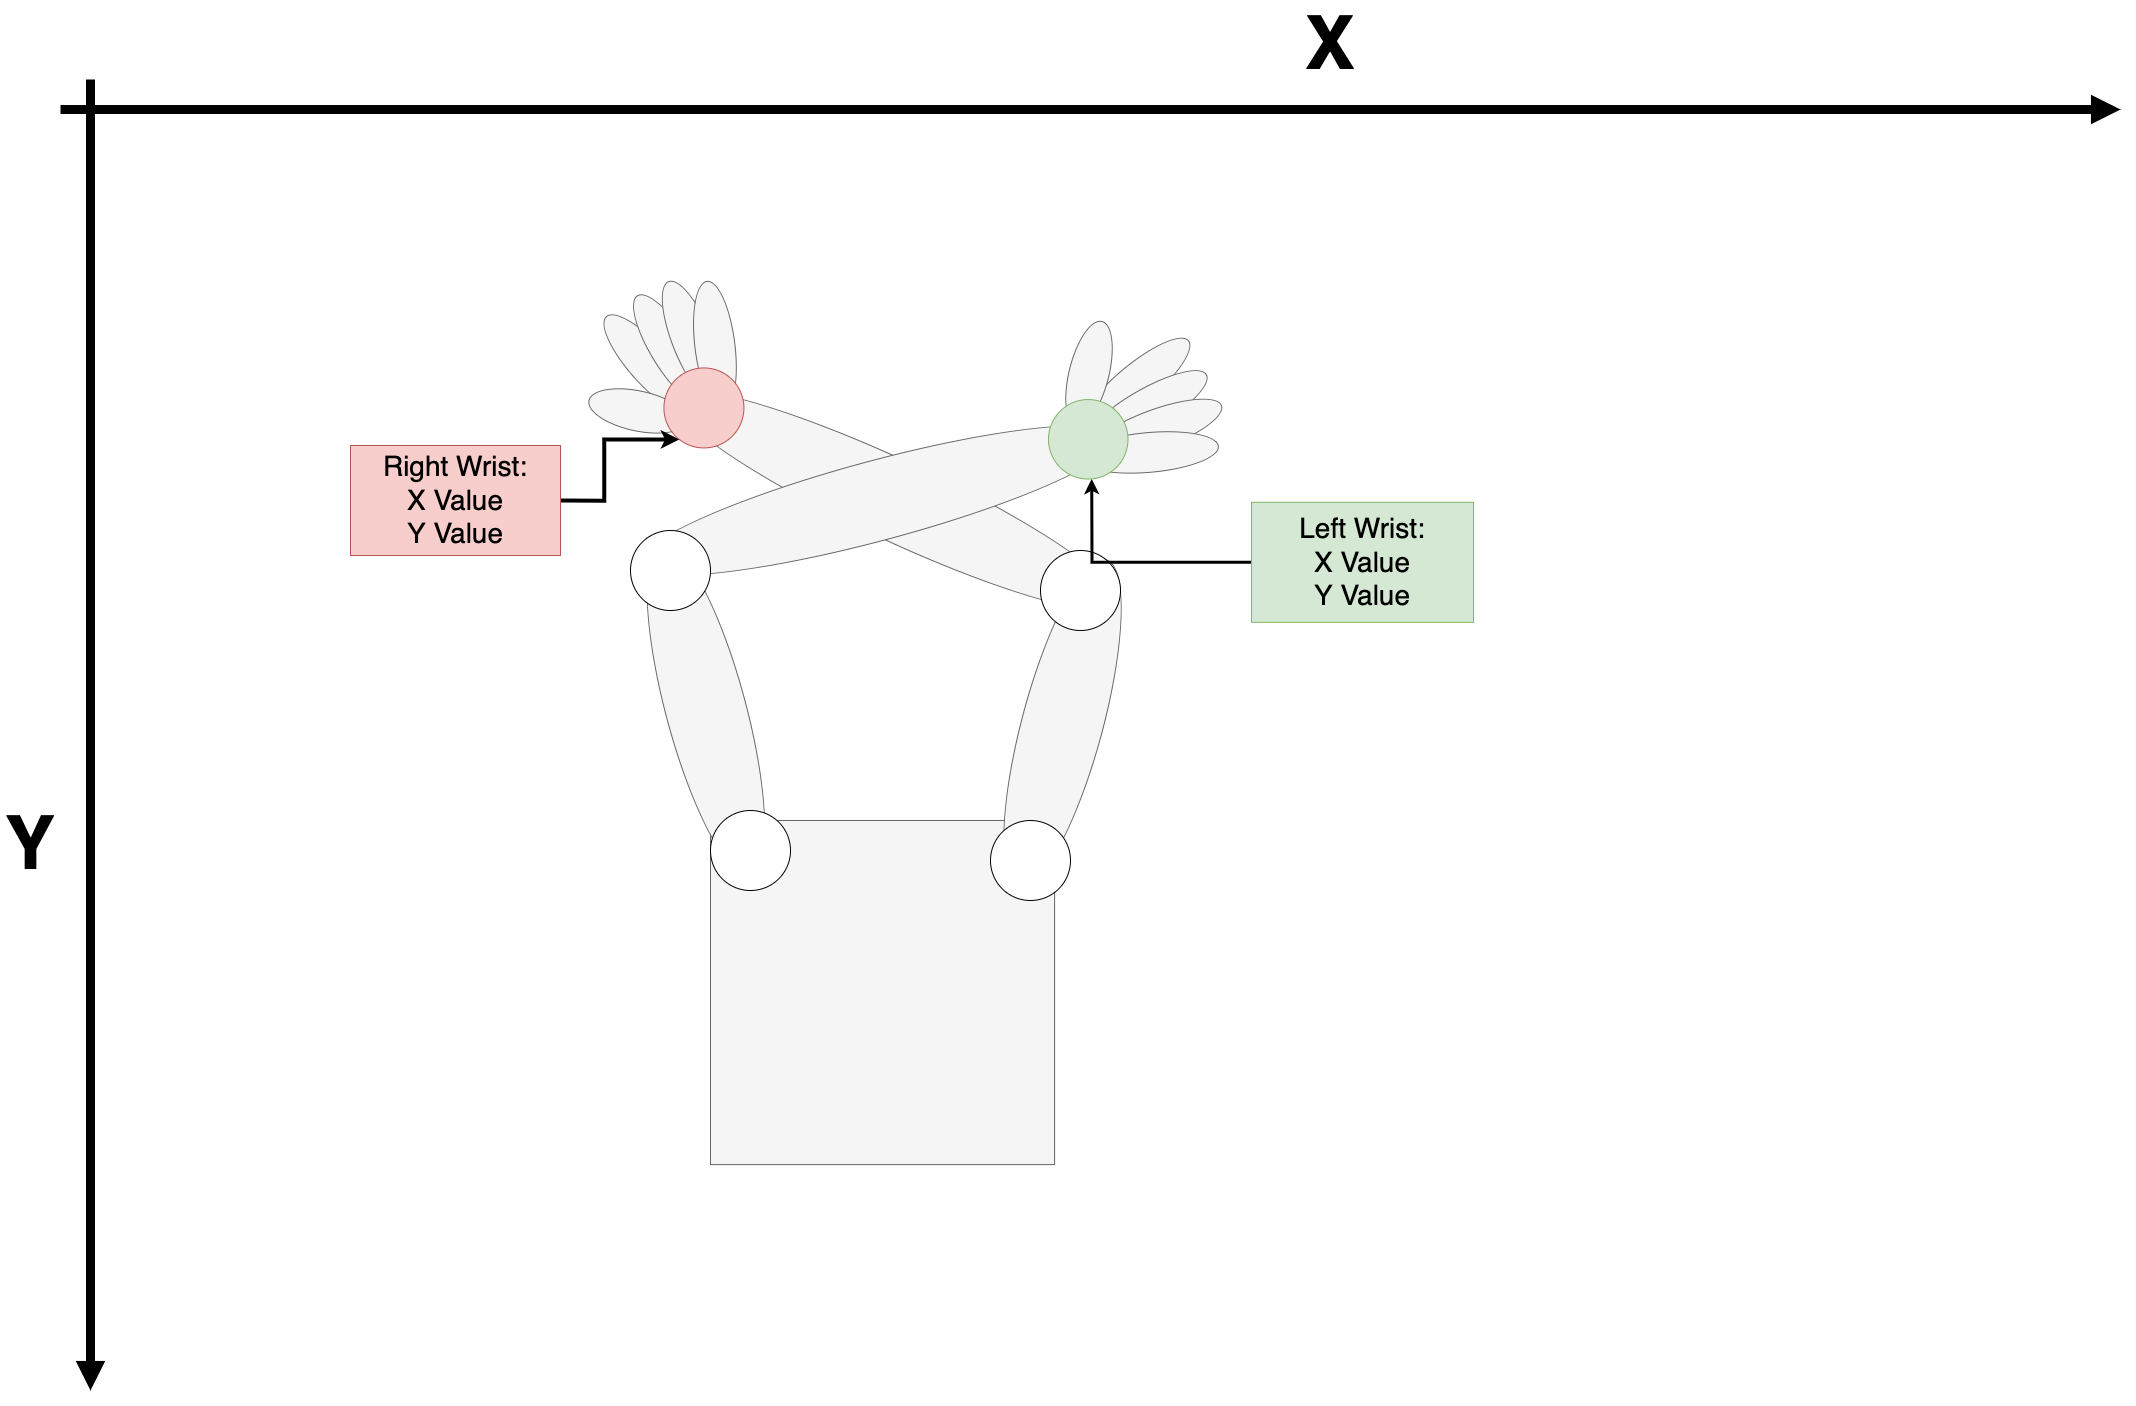
\includegraphics[width=\textwidth]{images/arms_crossed.png}
	\caption{Pictogram of the pose "arms crossed"}
	\label{arms_crossed}
\end{figure}
\subsection{Autonomous Movement}

\begin{figure}[H]
	\centering
	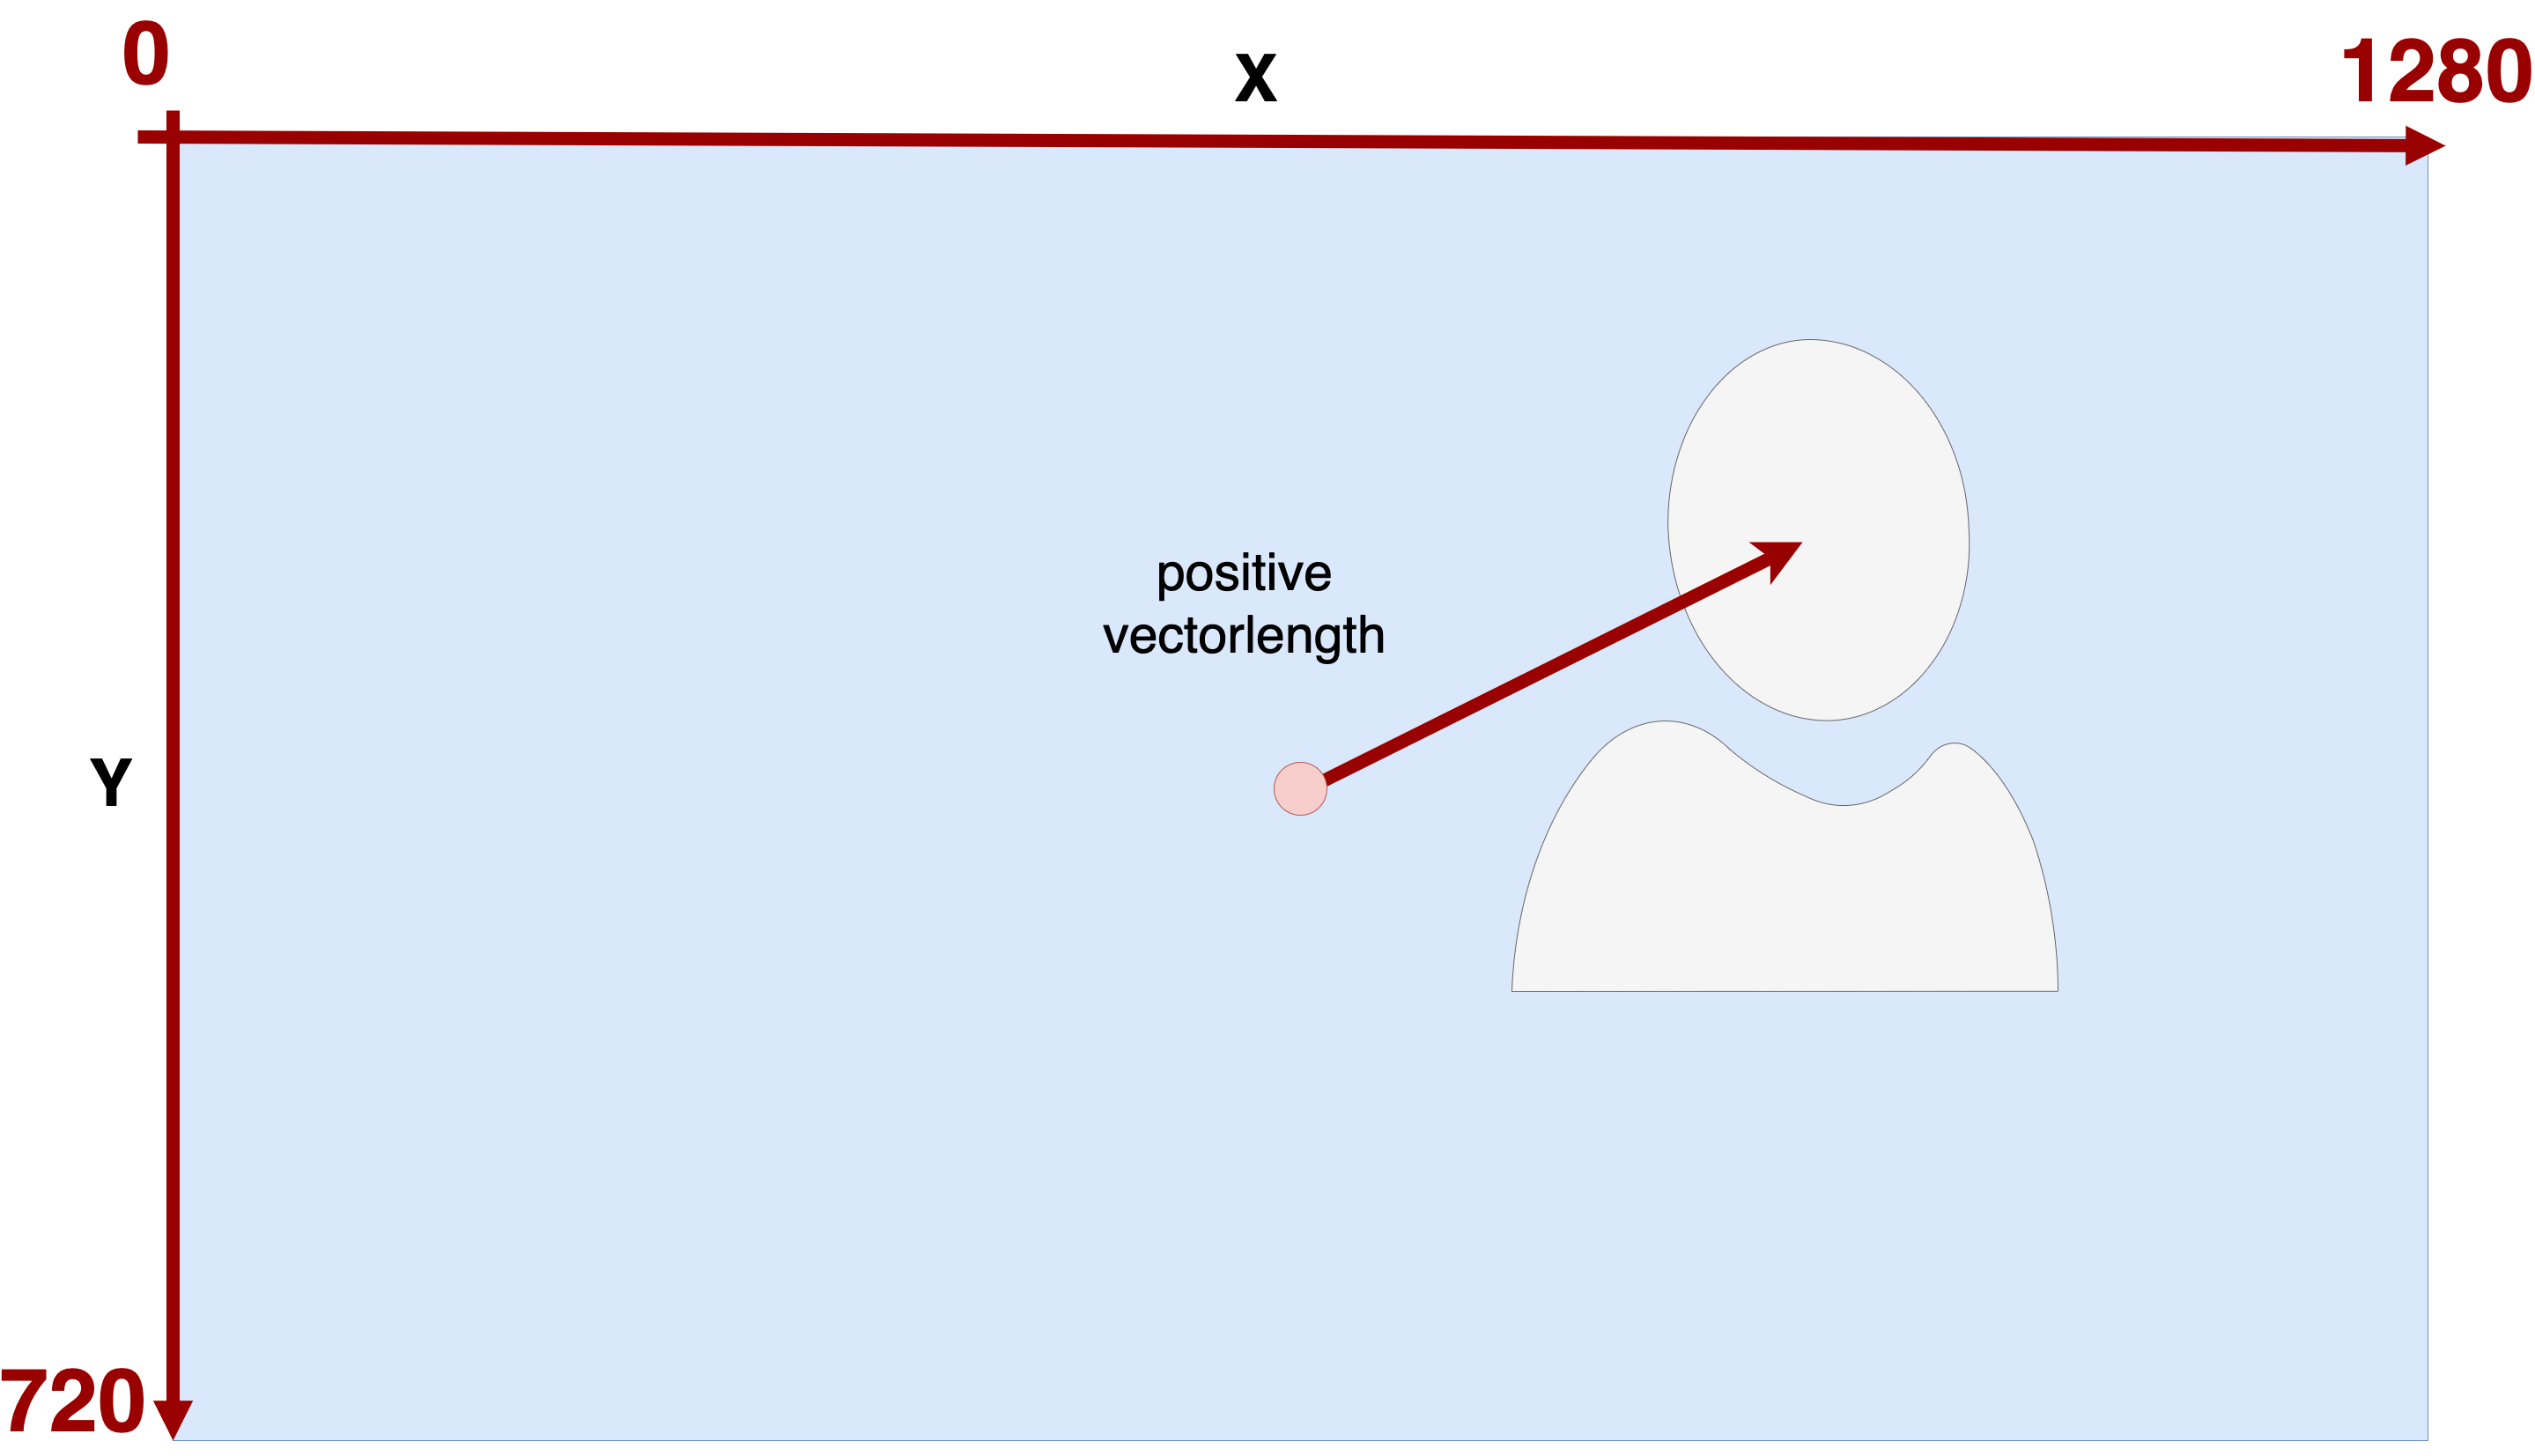
\includegraphics[width=\textwidth]{images/positive_vector_length.png}
	\caption{Movement if the vectorlength is positive}
	\label{positive_vectortlength}
\end{figure}

\begin{figure}[H]
	\centering
	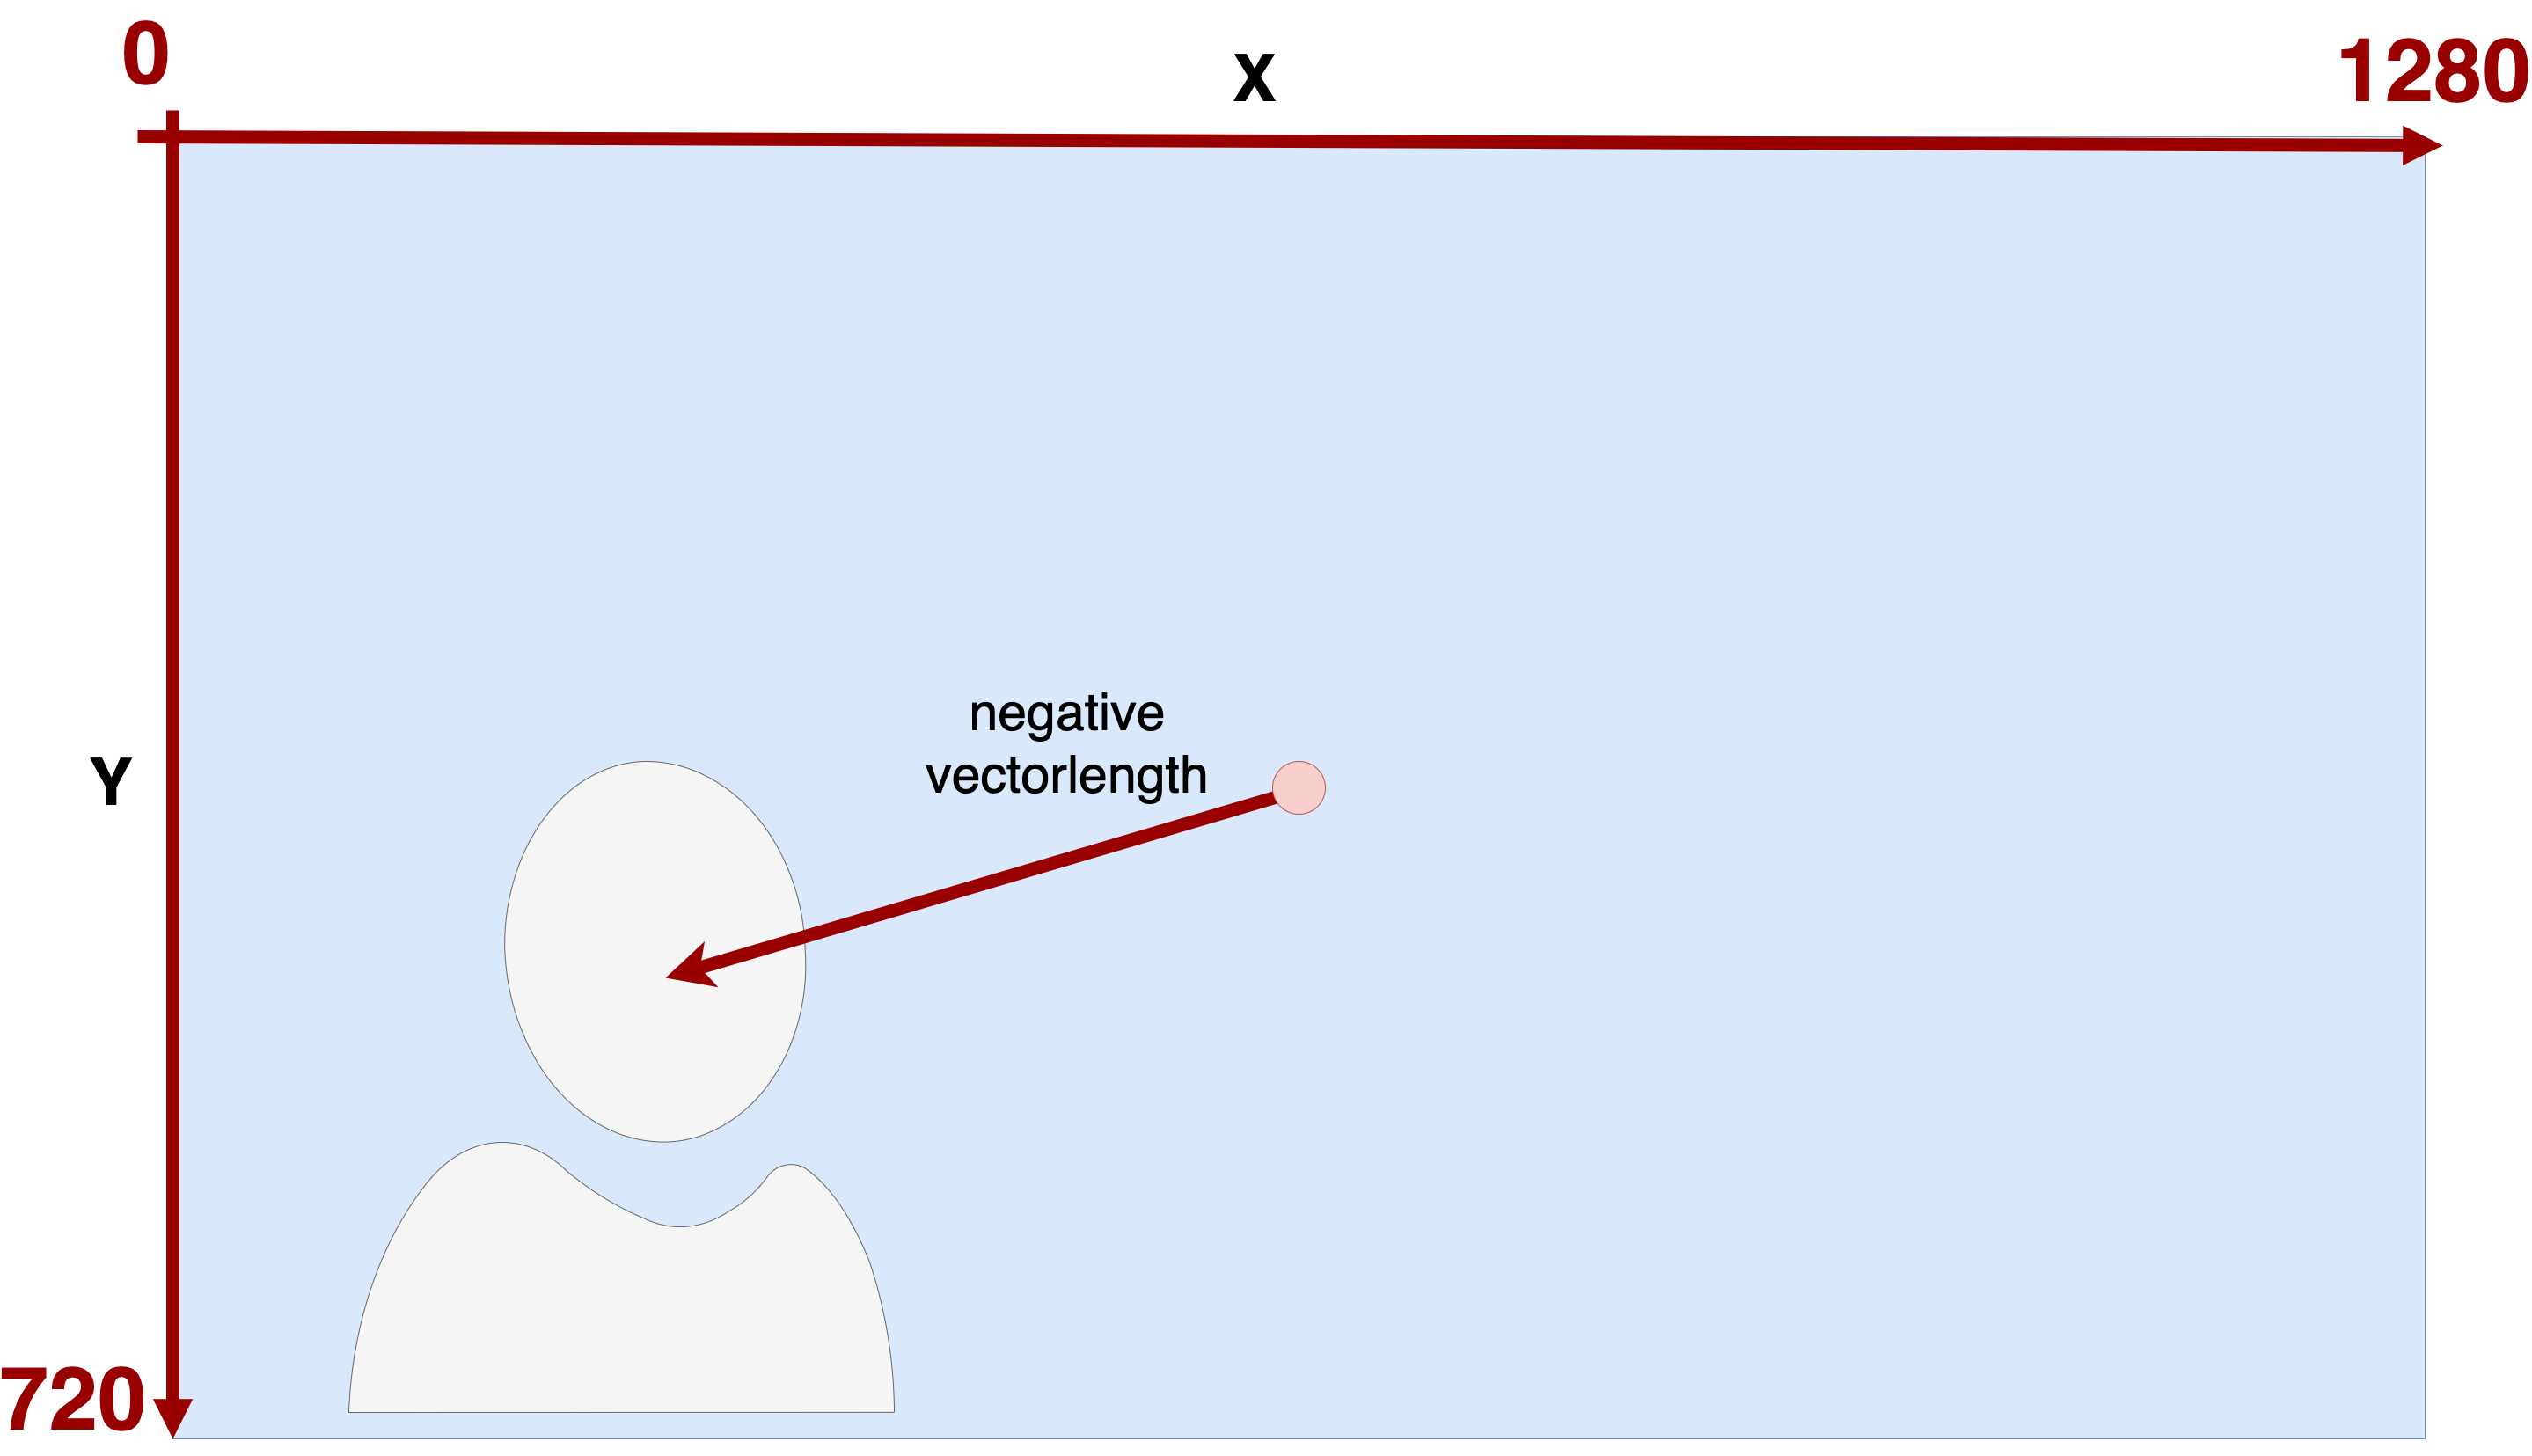
\includegraphics[width=\textwidth]{images/negative_vector_length.png}
	\caption{Movement if the vectorlength is negativ}
	\label{negativ_vectortlength}
\end{figure}

\begin{figure}[H]
	\centering
	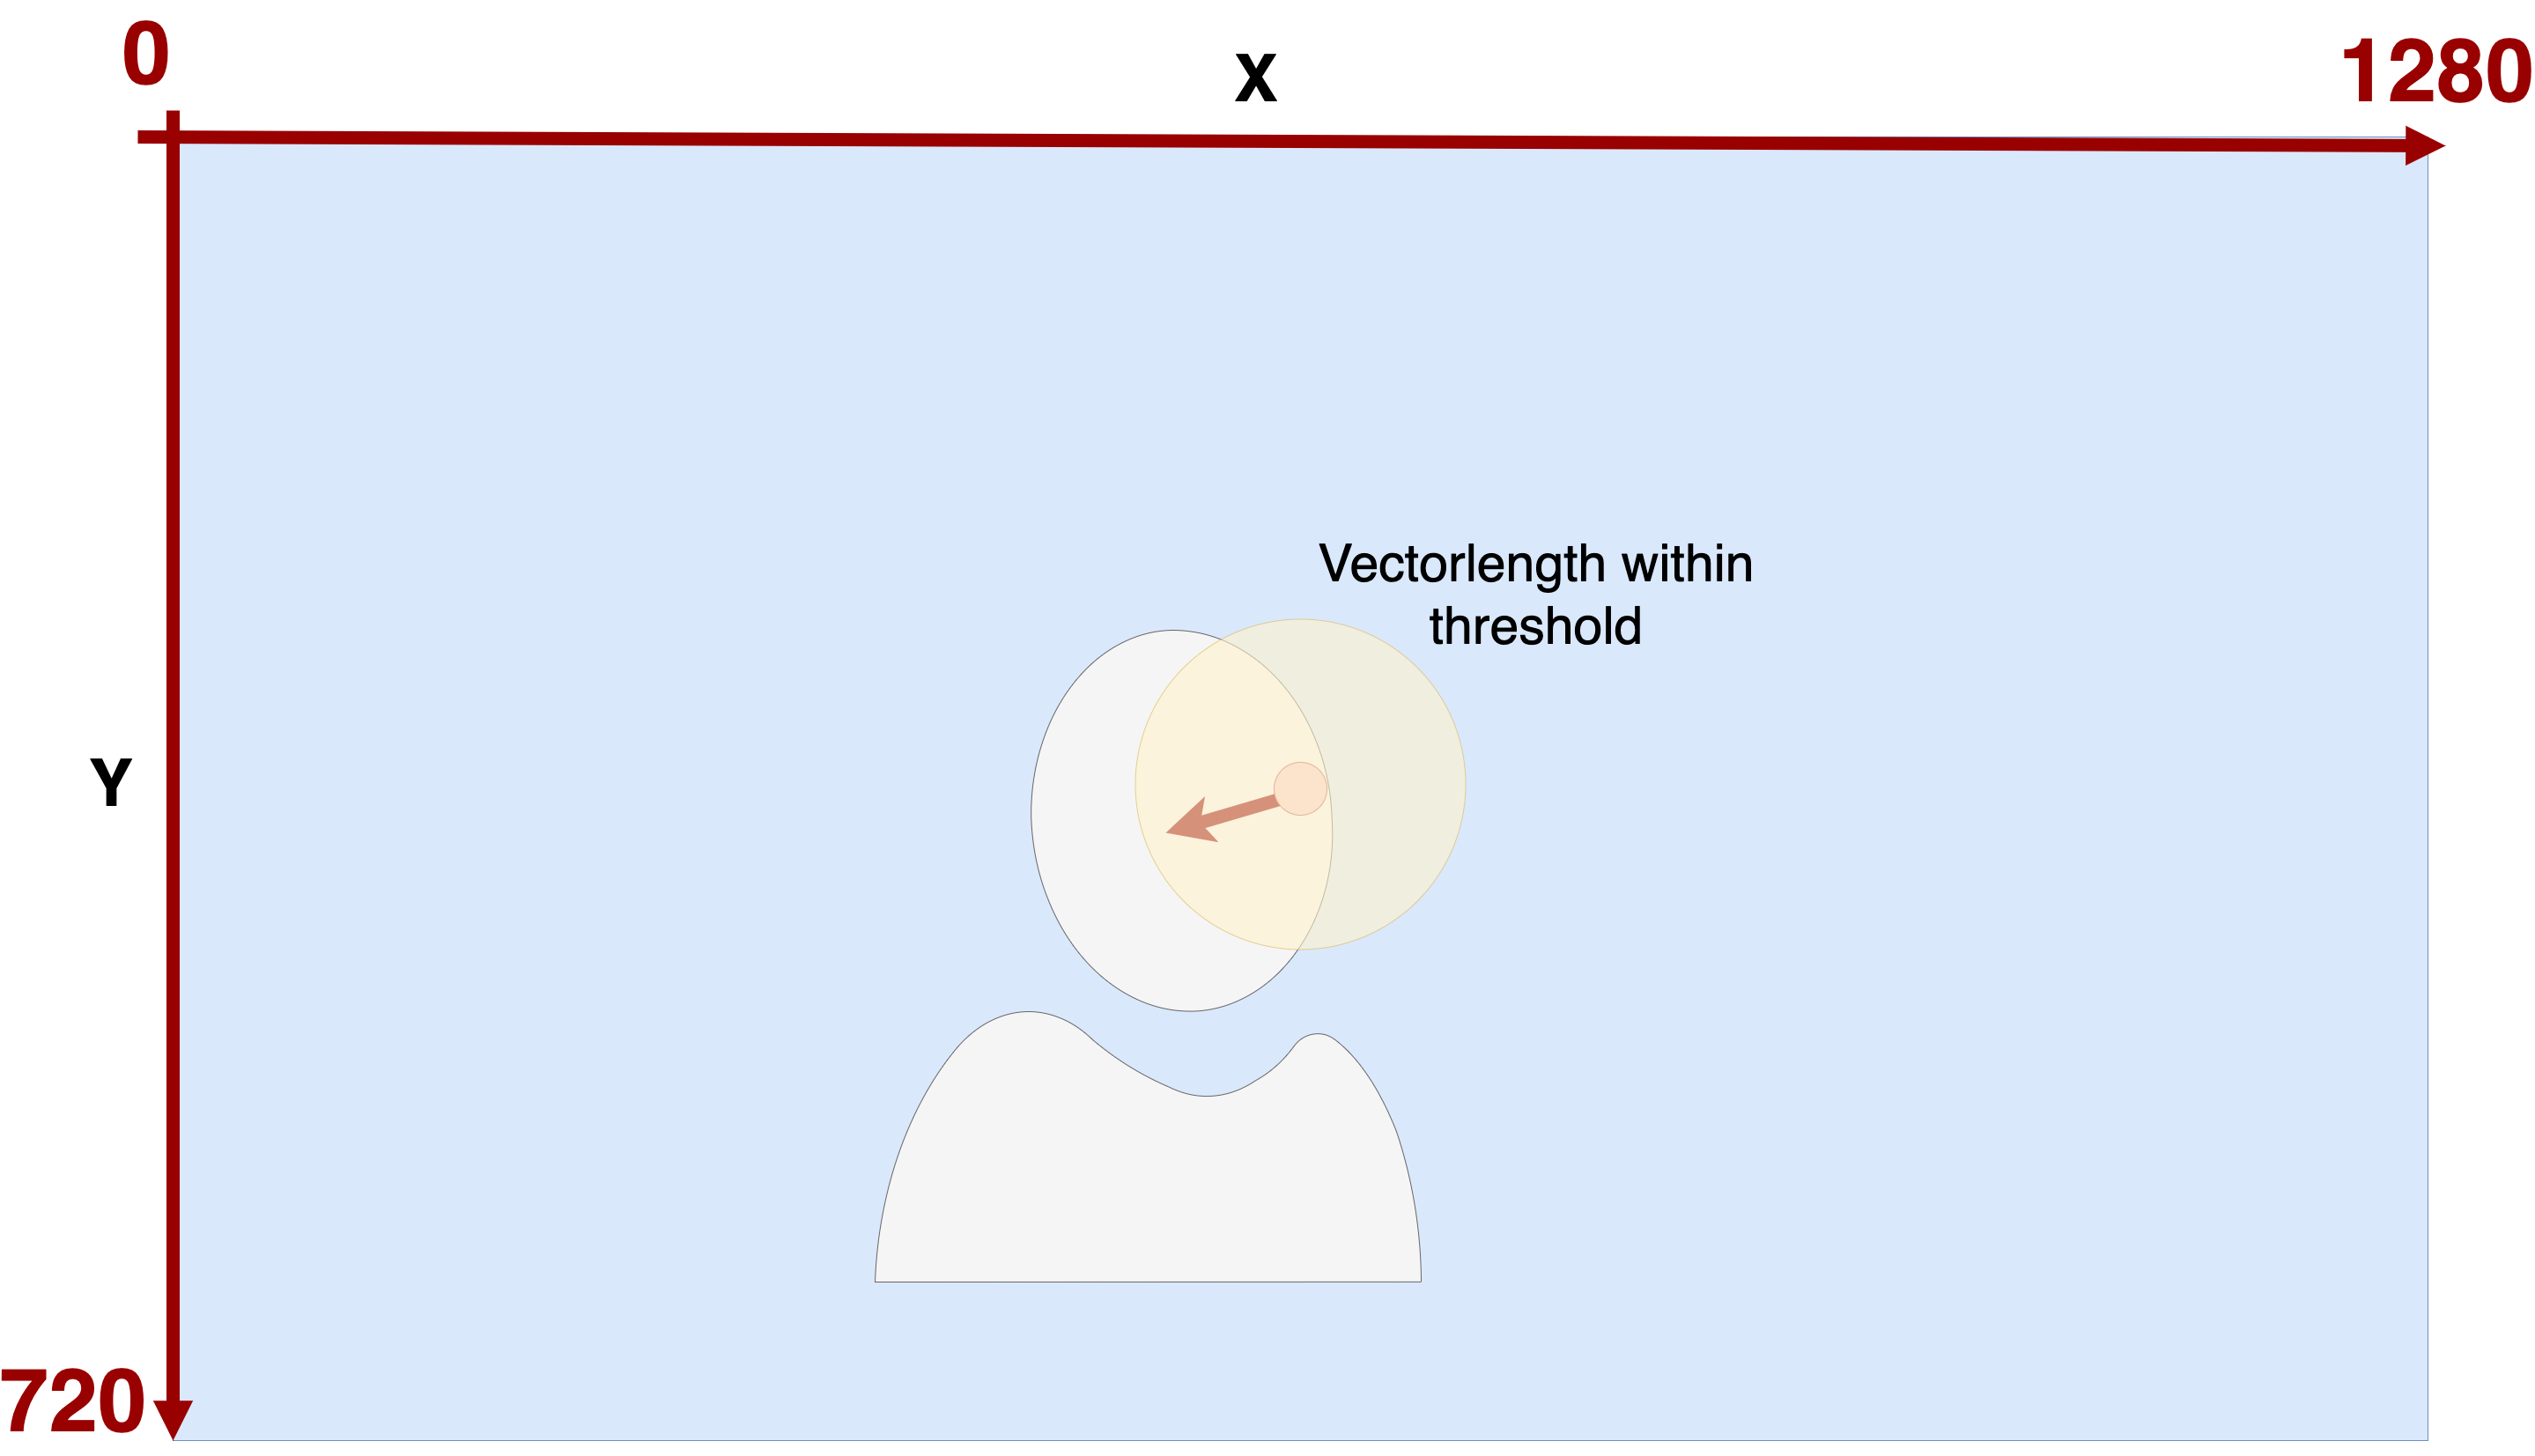
\includegraphics[width=\textwidth]{images/vectorlength_between_treshold.png}
	\caption{Drone is stalling if vectorlength is within the treshold}
	\label{vectorlength_treshold}
\end{figure}



\pagebreak
%%%%%%%%%%%%%%%%%%%%%%%%%%%%%% Conclusion
\section{Conclusion}
In the final test, the drone held its position surprisingly well considering the simplicity of the algorithm.
The implemented poses were recognized flawlessly and there is no problem with the ambiguity of certain poses, which can only be achieved by unnatural arm movements.
This does not occur in practical use.
The autonomous flight capability of the drone was also good, even if the tresholds are not optimally adjusted, which manifests itself as oversteering in the movements.


\pagebreak
%%%%%%%%%%%%%%%%%%%%%%%%%%%%%% Improvements
\section{Improvements}
\textbf{Keeping the drone the same distance:}\\
The drone is currently not able to move in z direction. First approaches where made by calculating
shoulder length and keep distance between a set threshold. 
This resulted not in the desired outcome since it would only work if the person stands in a completly frontal pose.
If shoulders are twisted in, the algorithm would make a wrong distance correction.
\\\\
Additionally to the landmarks x and y coordinates, BlazePose calculates a third z value 
which indicates the depth of the landmark to the center of the hips. 
With this information it should be possible to accurately determine the drones distance to the operator.
\\\\
\textbf{Fine tuning of thresholds and otehr settings:}\\
In the current setting, the drones performance is good enough to do 
all tasks mentioned in the previous chapters. Though sometimes thresholds are set to high, 
resulting in an overturn which lead to a corrective movement. This is preceived as a shaking of the drone.
By tuning the setting parameters a smoother experience could be achieved.
\\\\
\textbf{Operating the drone via App:}\\
Among other things BlazePose was chosen because it works very efficiently.
Ultimately the drone acts as an selfie drone you would take on a trip or walk, 
thus the algorithm should work on a portable device, preferably a mobile phone.\\
The paper states\cite{BlazePosePaper} that BlazePose is able to perform up to 44fps on a Google Pixel 3.
Thus it would be possible to design an Application which can handle the functions implemented in this project. 

\pagebreak
\listoffigures
\pagebreak
\printbibliography[heading=bibintoc]
\pagebreak
\lstlistoflistings
\pagebreak
\lstinputlisting[language=Python,caption=Main.py]{../../source/Main.py}
\lstinputlisting[language=Python,caption=Controller.py]{../../source/Controller.py}
\lstinputlisting[language=Python,caption=Constants.py]{../../source/Constants.py}
\lstinputlisting[language=Python,caption=PoseDetection.py]{../../source/Pose.py}
\end{document}